\section{Calculating Rotations}
\Cref{ssc:xy_angles} defined how a 2D image is analysed to find the difference, in degrees, between a centred vector and the location of an object. The following section explains how this centred vector is rotated to intersect the targeted object in 3D space.

The angles are found on the x- and y-axis meaning the rotations will be performed on these axes. The rotation matrices needed are shown in \cref{eq:rotation_x} and \cref{eq:rotation_y} respectively.


\begin{equation}\label{eq:rotation_x}
\begin{bmatrix}
1 & 0 & 0 \\
0 & cos\theta & -sin\theta \\
0 & sin\theta & cos\theta \\
\end{bmatrix}
\end{equation}

\begin{equation}\label{eq:rotation_y}
\begin{bmatrix}
cos\theta  & 0 & sin\theta \\
0 & 1 & 0 \\
-sin\theta & 0 & cos\theta \\
\end{bmatrix}
\end{equation}

The rotation matrices rotate vectors counter clockwise from their original direction. \Cref{fig:signed_angles} shows how these rotations are represented in the images.
\begin{figure}[H]
    \centering
    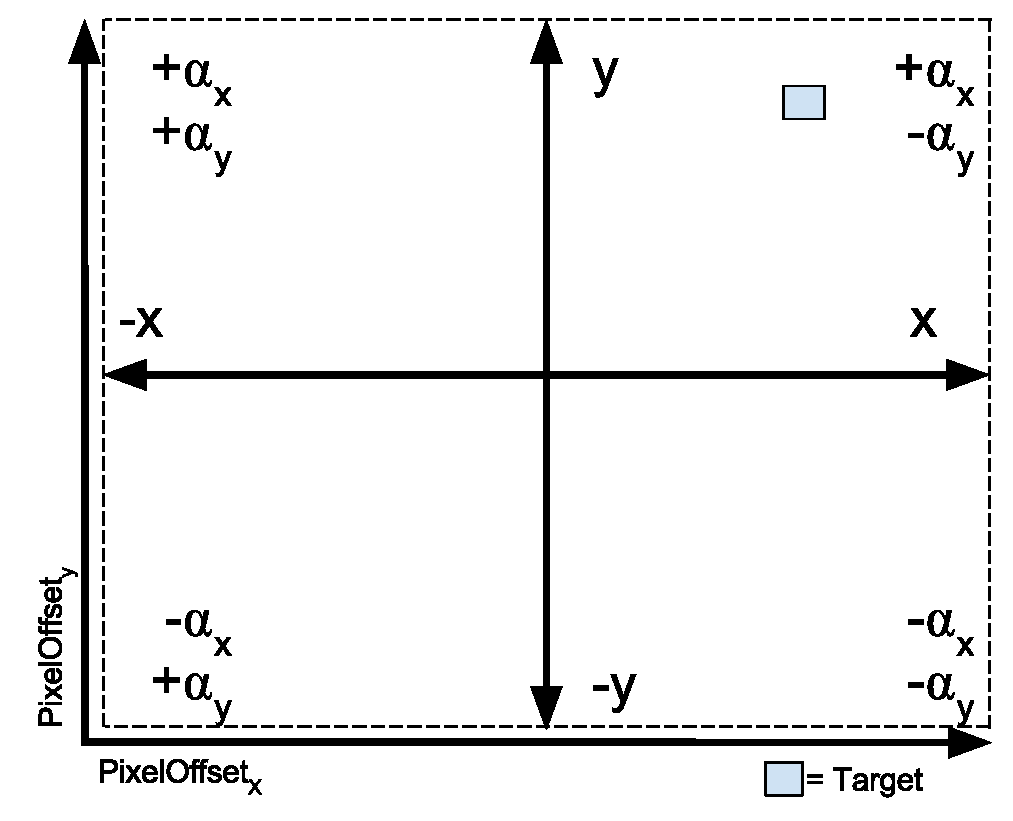
\includegraphics[scale=.65]{graphics/signed_angles.eps}
    \caption{Example showing angle values, depending on graph quadrants}
    \label{fig:signed_angles}
\end{figure}

Looking at the first quadrant containing the target, the rotation around the x-axis must be a counter clockwise rotation from center origin, which is why the degrees must be positive. \Cref{eq:offset-y_fov} returns positive values when target is greater than half the height of the image, therefore, this equation returns the wanted result. \Cref{eq:offset-x_fov} however, returns negative values when target is on the left side of the image and positive values when the target is on the right side of the image, which is opposite from the wanted behaviour. This behaviour is easily achieved however, by negating the result of \cref{eq:offset-x_fov}, resulting in \cref{eq:offset-x_opt}
\begin{align}
-\left(\frac{Offset_X - 0.5 * Width}{0.5 * Width}\right)*F_x*0.5
\label{eq:offset-x_opt}
\end{align}
The following section gives an example of finding the angle derivations and then rotating the lens' centre vector to cut the target's position.

\section{Example of Calculations}
A picture is taken with a camera and an object is defined to be located at the first quadrant of the image, with a pixel offset of $(x,y)=(500,400)$, the size of the image is $640x480$ $pixels$ and the \gls{fov} of the camera is $62\degree$. This information is inserted into \cref{eq:offset-y_fov} and \cref{eq:offset-x_opt}, giving:
\begin{align}
-\left(\frac{500 - 0.5 * 640}{0.5 * 640}*F_x*0.5\right) = -17.44\degree
\label{eq:ex_offset-x_opt}
\end{align}
\begin{align}
\frac{400 - 0.5 * 480}{0.5 * 480}*F_y*0.5 = 20.67\degree
\label{eq:ex_offset-y}
\end{align}

Next is to rotate the wanted vector which is the camera lens' vector previously defined as
$\left[\!\begin{array}{c}
0\\
0\\
-1
\end{array}\!\right] $
 it has to be rotated $20.67\degree$ around the x-axis and $-17.44\degree$ around the y-axis. which is shown in \cref{eq:rotation_on_x_and_y_part1} and \cref{eq:rotation_on_x_and_y_part2}.
\begin{equation}\label{eq:rotation_on_x_and_y_part1}
\begin{bmatrix}
1 & 0 & 0 \\
0 & cos(20.67) & -sin(20.67) \\
0 & sin(20.67) & cos(20.67)
\end{bmatrix}
\begin{bmatrix}
0 \\
0 \\
-1
\end{bmatrix}
=
 \begin{bmatrix}
0 \\
0.353\\
-0.936
\end{bmatrix}
\end{equation}
\begin{equation}\label{eq:rotation_on_x_and_y_part2}
\begin{bmatrix}
cos(-17.44)  & 0 & sin(-17.44) \\
0 & 1 & 0 \\
-sin(-17.44) & 0 & cos(-17.44)
\end{bmatrix}
\begin{bmatrix}
0 \\
0.353\\
-0.936
\end{bmatrix}
=
 \begin{bmatrix}
0.280 \\
0.353 \\
-0.893
\end{bmatrix}
\end{equation}
$\left[\!\begin{array}{c}
0.280 \\
0.353 \\
-0.893
\end{array}\!\right] $
is the vector in the local coordinate system of the camera, which cuts the object. This vector has to be transmuted into the global coordinate, so the actual position of the object can be calculated for the 3D space.
